\section{Design a control circuit for described operation below:}
\subsection{Push button start.}
\subsubsection{Motor 1 (AC1phase), Motor2(3phase) run in star mode, after 5s motor 1 change direction, motor 2 change from star to delta, motor 3 start running.}
Motor 1 (AC1phase), Motor 2 (3phase) run in star mode:
\begin{figure}[H]
    \centering
    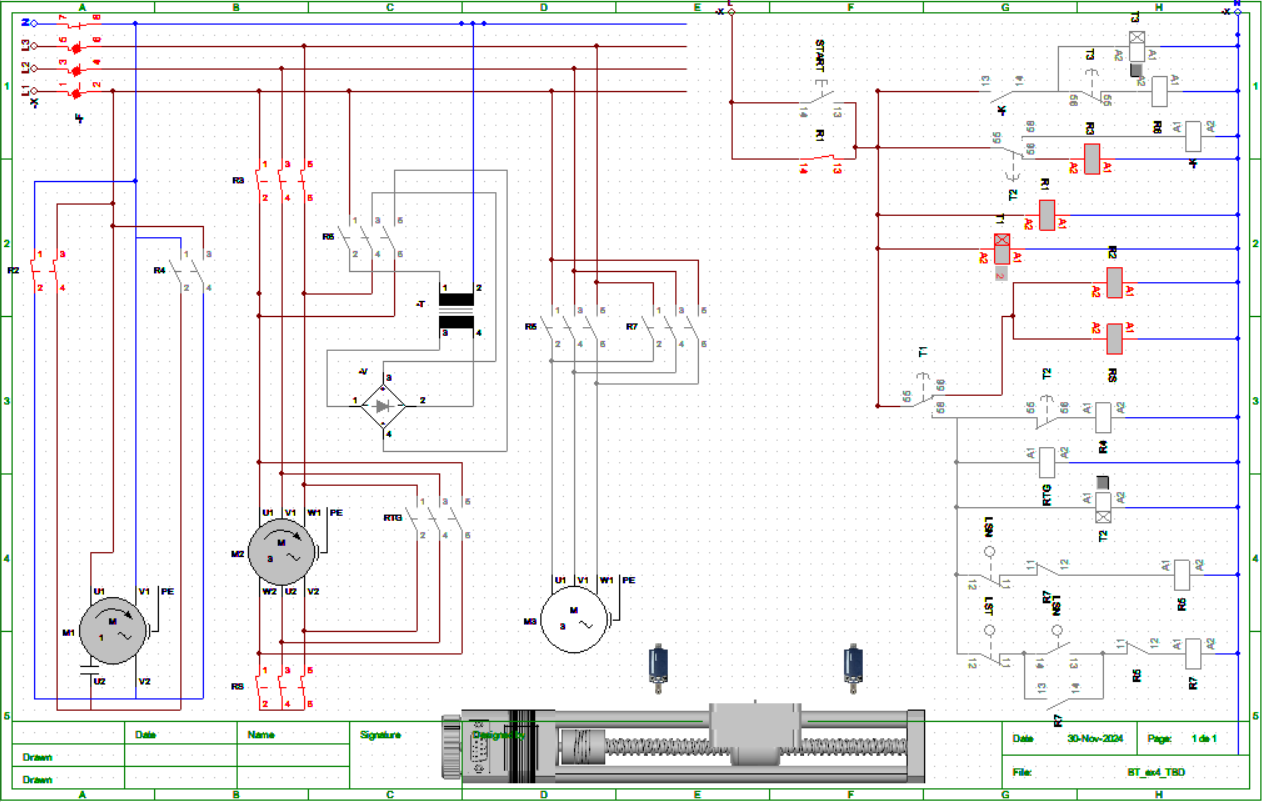
\includegraphics[width=1\textwidth]{pictures/1a.png}
\end{figure}
\cleardoublepage
After 5s motor 1 change direction, motor 2 change from star to delta, motor 3 start running:
\begin{figure}[H]
    \centering
    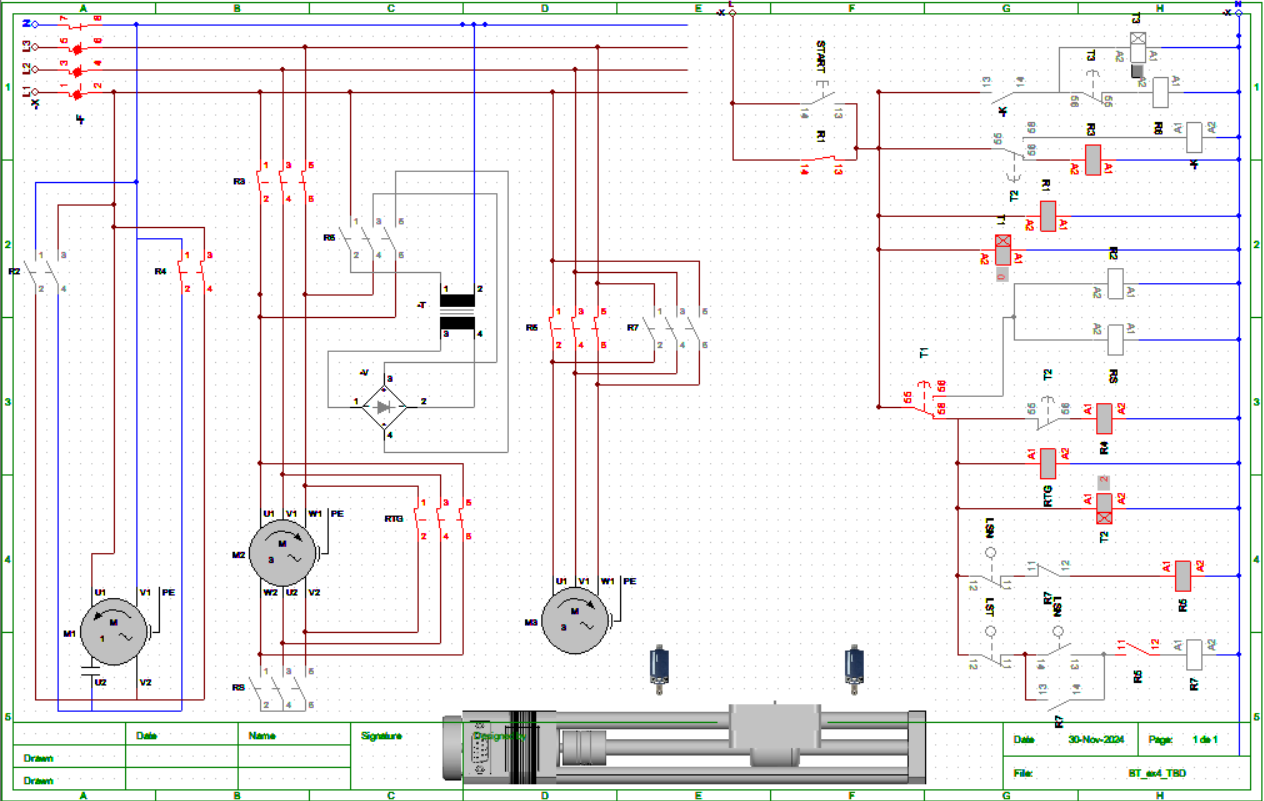
\includegraphics[width=1\textwidth]{pictures/1b.png}
\end{figure}
\cleardoublepage
\subsubsection{Motor 3 (3phase) runs from left to right then meets a limit switch then return to right then loop again,  while in 5s later motor1 stops and motor2 stop (kinematic).}
Motor 3 (3phase) runs from left to right then meets a limit switch then return to right then loop again:
\begin{figure}[H]
    \centering
    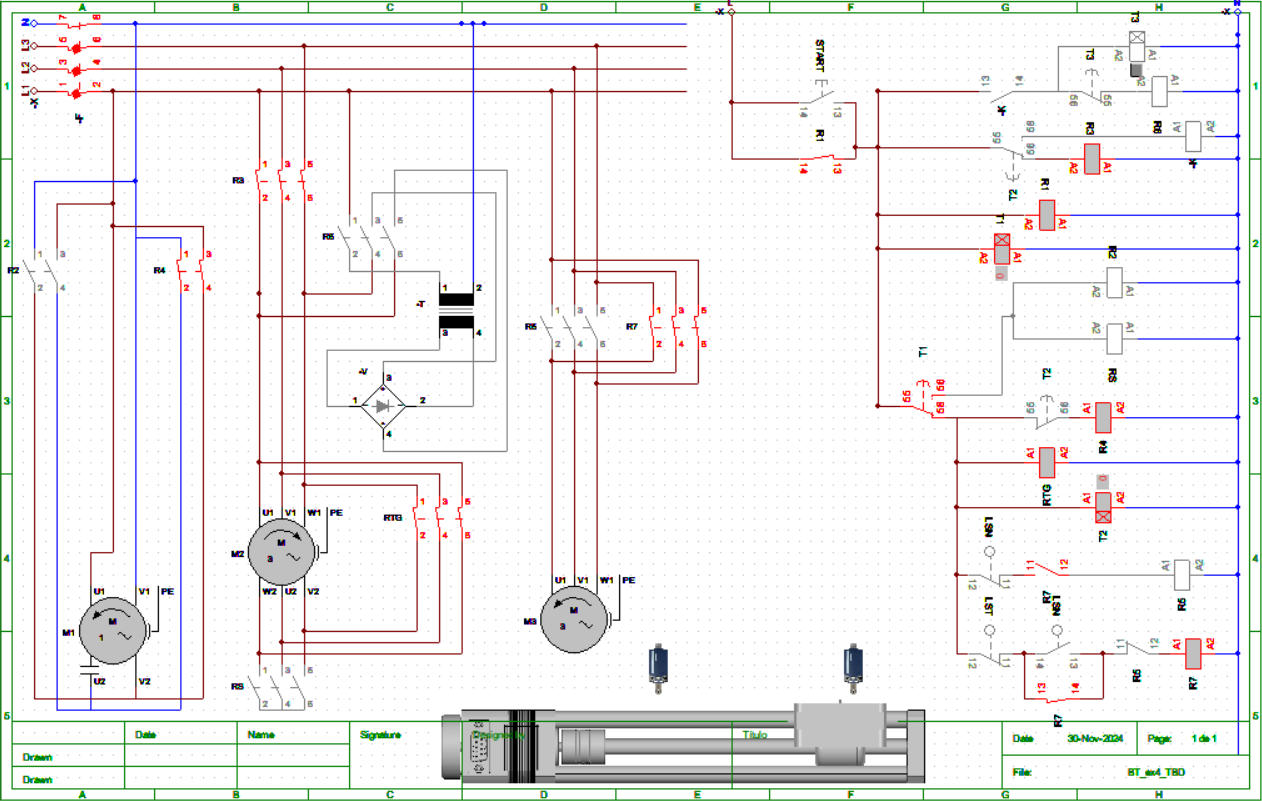
\includegraphics[width=1\textwidth]{pictures/1c.png}
\end{figure}
\cleardoublepage
In 5s later motor 1 stops and motor 2 stop (kinematic):
\begin{figure}[H]
    \centering
    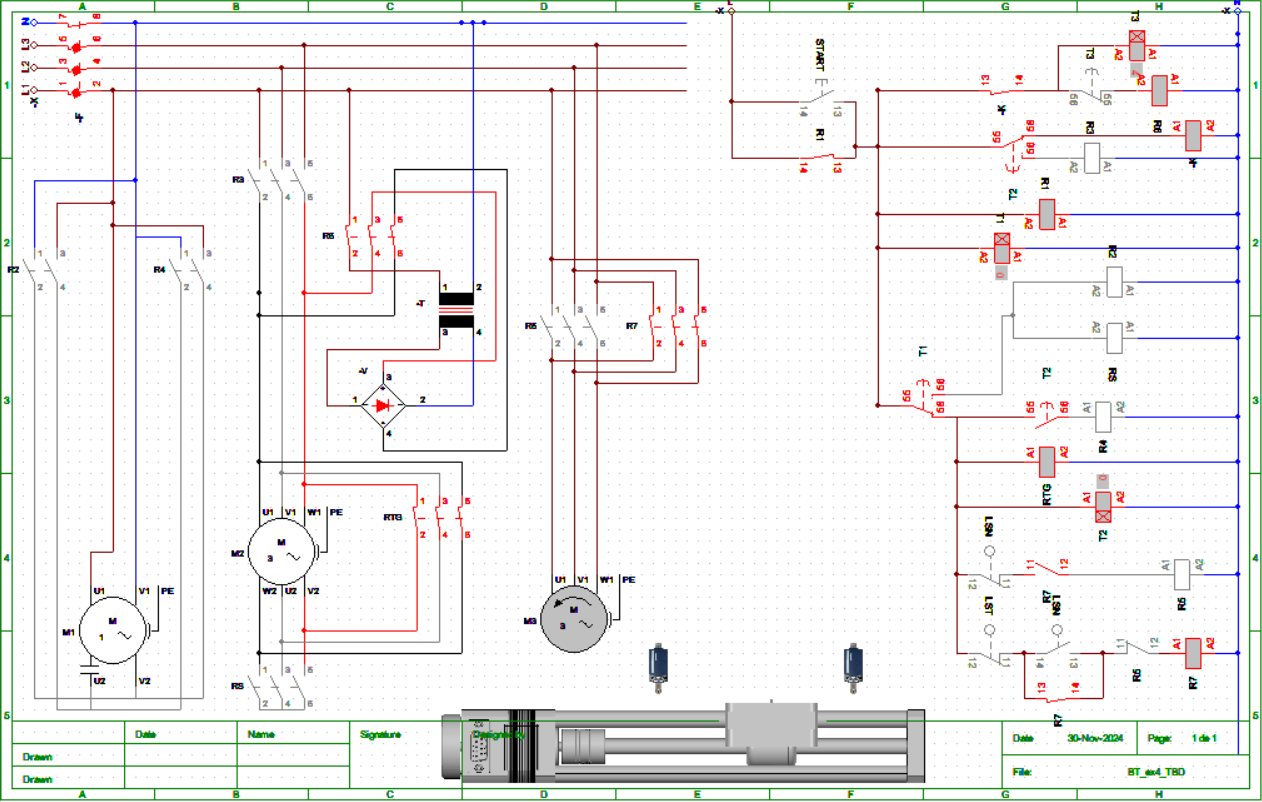
\includegraphics[width=1\textwidth]{pictures/1d.png}
\end{figure}
\cleardoublepage
\subsection{Circuit have emergency stop button.}
\subsubsection{Before the emergency stop button is pressed}
\begin{figure}[H]
    \centering
    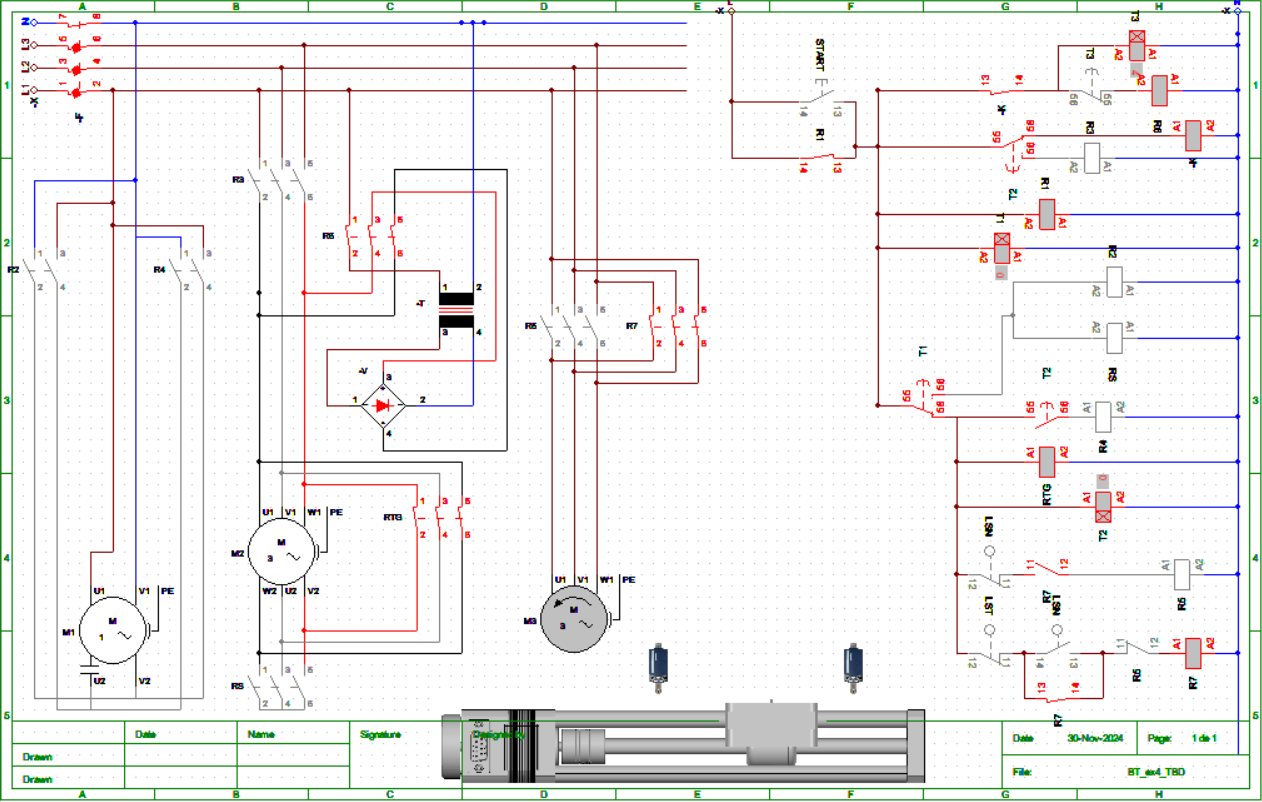
\includegraphics[width=1\textwidth]{pictures/1d.png}
\end{figure}
\cleardoublepage
\subsubsection{After the emergency stop button is pressed}
\begin{figure}[H]
    \centering
    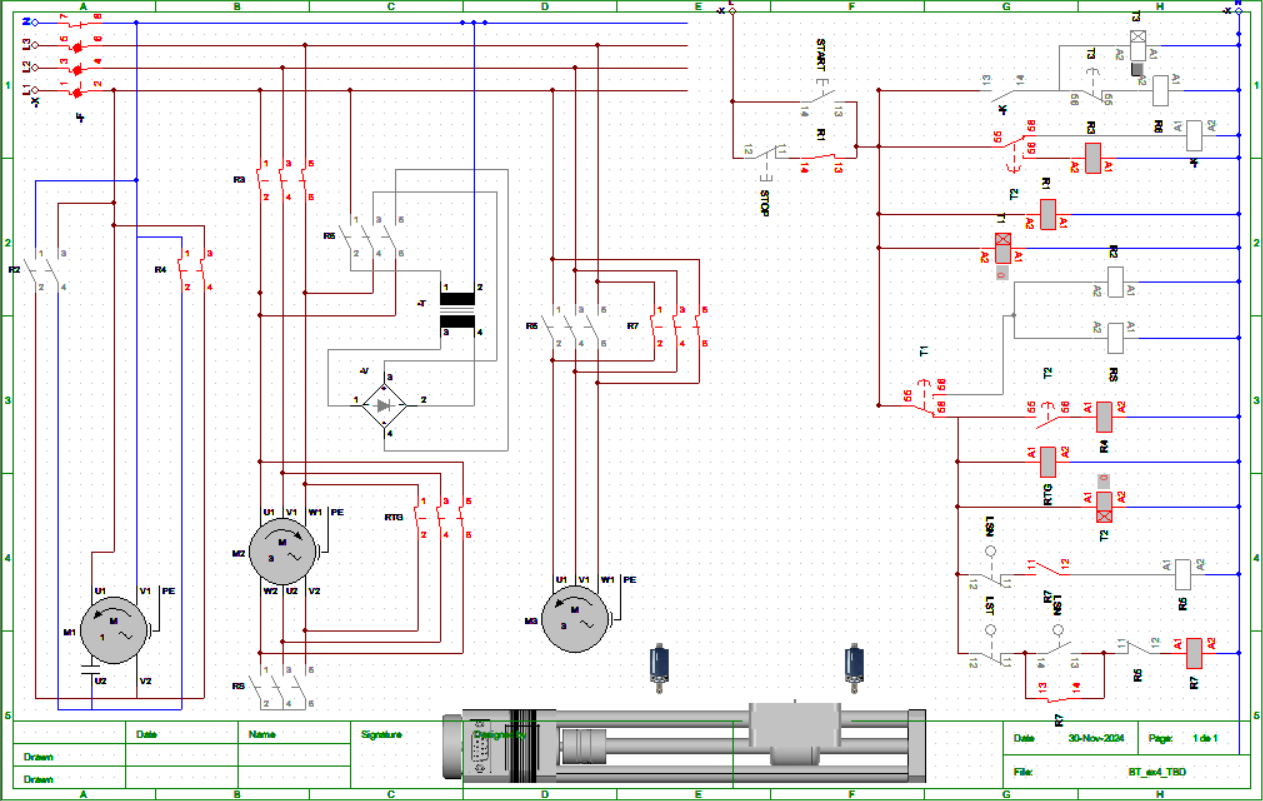
\includegraphics[width=1\textwidth]{pictures/1e.png}
\end{figure}
$\Rightarrow$ After the emergency stop button is pressed, all motors stop immediately and will not reactivate until the start button is pressed.
\cleardoublepage